\documentclass[	%draft, % To display over/unterfull hboxes
				a4paper, % use DIN A4 Paper
				onecolumn, % Only one Column of text
				oneside, % Pint only right sides
				titlepage, % Print a titlepage
				openany, % Open new chapter on any page
				12pt] % Text size
				{article}

\usepackage[left=3cm,right=3cm,top=3cm,bottom=3cm]{geometry} % Page margins
\usepackage[english, ngerman]{babel} % Better line breaking
\usepackage[utf8]{inputenc} % Utf8 recognition
\usepackage[T1]{fontenc} % Translate from latex code to draw font
\usepackage{lmodern} % Bolder font
\usepackage{graphicx} % Display images
\usepackage{fancyhdr} % Header/footer
\usepackage[pdfborder={0 0 0}]{hyperref} % Links without visible lines
\usepackage[table]{xcolor} % Get the color in the table
\usepackage{pdflscape} % Get the table into landscape mode
\usepackage[lastpage]{zref} % Set a lable on the last page
\usepackage{listings} % Display formatted code
\usepackage{makeidx} % Generates the index
\usepackage{acronym} % Generates the list of abbreviations
\usepackage{multicol} % List of abbreviations with two columns
\usepackage{bibgerm} % BibTex German Style DIN 1505
\usepackage{longtable} % Multi page tables
\usepackage{subfigure} % Multiple gaphics in one figure
\usepackage{setspace} % set line spacing
\usepackage{amsmath} % Improved Math mode
\usepackage{amsfonts} % Improved Math mode
\usepackage{amssymb} % Improved Math mode
\usepackage{mathtools} % Improved Math mode
\usepackage{csquotes}
\usepackage{upquote}
%\usepackage{underscore}

% Tell LaTeX to generate an index
\makeindex

% No indent @ line start
\parindent 0pt

% The bibstyle
% gerplain is for only numbers in alphabetic order
% geralpha is for name+year in alphabetic order
\bibliographystyle{gerplain}

% Header
\pagestyle{fancy}

\fancypagestyle{plain}{}
\fancyhead[RO,RE]{Seite \thepage\ von\reallastpage}
\fancyhead[LO,LE]{\leftmark}

% Set the lastpage counter -1 
% So the statutory declaration is not part of the page counter
\makeatletter
\newcommand{\reallastpage}{
  \the \numexpr \zref@extractdefault{LastPage}{page}{0}-1\relax
}
\makeatother

% Header for starting section
\fancypagestyle{rightmark}{
	\fancyhead[LO,LE]{\rightmark}
}

% Empty footer
\cfoot{}

% Brake long url in cite
\def\UrlBreaks{\do\/\do-}

% Suppress clubs (Schusterjungen) 
\clubpenalty = 10000

% Suppress widows (Hurenkinder)
\widowpenalty = 10000

% Suppress widows in front of a formular
\displaywidowpenalty = 10000

% Macro for centering extreme wide tables/figures
\makeatletter
\newcommand*{\Centerfloat}{%
  \parindent \z@
  \leftskip \z@ \@plus 1fil \@minus \textwidth
  \rightskip\leftskip
  \parfillskip \z@skip}
\makeatother

% Change the text from the list of listings
\addto\captionsngerman{\renewcommand{\bibname}{Literatur- \& Quellenverzeichnis}}

%------------------------------------------------------------------------------
% Macro for two abstracts on one page:
%------------------------------------------------------------------------------

\newenvironment{Abstract}{
  \vspace*{\fill}
  \begin{center}%
    \bfseries\abstractname
  \end{center}}%
  {\vfill}

%------------------------------------------------------------------------------
% Macro for reusing some text:
%------------------------------------------------------------------------------

% Use to define some text and then re use the very same text
% \ref{sth:bla}
% \textlabel{Something AAA}{sth:bla}
\makeatletter
\newcommand*{\Textlabel}[2]{%
  \edef\@currentlabel{#1}% Set target label
  \phantomsection% Correct hyper reference link
  #1\label{#2}% Print and store label
}
\makeatother

%------------------------------------------------------------------------------
% Macros for the list of abbreviations:
%------------------------------------------------------------------------------

% To wirte the text only once
\newcommand*{\ListOfAbbreviations}{Abkürzungsverzeichnis}

% use reversed form
\makeatletter
\renewcommand*{\@acf}[1]{%
\ifAC@footnote
\acsfont{\AC@acs{#1}}%
\footnote{\AC@placelabel{#1}\hskip\z@\AC@acl{#1}{} }%
\else
\acsfont{% Orig:\acffont
\AC@placelabel{#1}\hskip\z@\AC@acs{#1}%Orig: \AC@acl{#1}
\nolinebreak[3] %
\acfsfont{(\acffont{\AC@acl{#1}})}%Orig: (\acsfont{\AC@acs{#1}})
}%
\fi
\ifAC@starred\else\AC@logged{#1}\fi
}
\makeatother

%------------------------------------------------------------------------------
% Macros for the the Index:
%------------------------------------------------------------------------------

% The thickness of the line between the columns of the index and the list of 
% Abbreviations; 0.4 pt is the LaTeX standart
\newcommand*{\LineThickness}{0.4 pt}

% Display twoculums with  vertical seperator line
\makeatletter
\renewenvironment{theindex}
  {\if@twocolumn
      \@restonecolfalse
   \else
      \@restonecoltrue
   \fi
   \setlength{\columnseprule}{\LineThickness} % Thikness of the columnseprule
   \setlength{\columnsep}{35 pt}
   \begin{multicols}{2}[\chapter*{\indexname}] % Amount of Columns
   \markboth{\MakeUppercase\indexname}%
            {\MakeUppercase\indexname}%
   \thispagestyle{plain}
   \setlength{\parindent}{0pt}
   \setlength{\parskip}{0pt plus 0.3pt}
   \relax
   \let\item\@idxitem}%
  {\end{multicols}\if@restonecol\onecolumn\else\clearpage\fi}
\makeatother

%------------------------------------------------------------------------------
% Macros for table colors and longtables:
%------------------------------------------------------------------------------

% Table gray row
\newcommand*{\Grayrow}{\rowcolor{gray!35}}

% Table red cell
\newcommand*{\Redcell}{\cellcolor{red!30}}

% Table green cell
\newcommand*{\Greencell}{\cellcolor{green!30}}

% Generates a small empty row in a longtable
\newcommand*{\EmptyRow}{\multicolumn{0}{l}{} \\[-9pt]}

% Needs to be @ the end of the longtable, 
% generates a caption with correct spacing
% @par1: the text of the caption
\newcommand*{\CaptionLongtable}[1]
	{\multicolumn{0}{l}{} \\[-3pt]\caption{#1}}
	
% Needs to be @ the end of the longtable, 
% generates a caption with correct spacing
% @par1: the text of the caption
% @par2: the text of the caption in the list of tables
\newcommand*{\CaptionLongtableS}[2]
	{\multicolumn{0}{l}{} \\[-3pt]\caption[#2]{#1}}

%------------------------------------------------------------------------------
% Macros for quotes:
%------------------------------------------------------------------------------

% A direct quote
% @par1: The quoted text
% @par2: The source where the text is from
% @par3: The page where the text is from
\newcommand*{\QuoteDirect}[3]{\QuoteM{\emph{#1}} \cite[#3]{#2}}

% A direct quote without page
% @par1: The quoted text
% @par2: The source where the text is from
\newcommand*{\QuoteDirectNoPage}[2]{\QuoteM{\emph{#1}} \cite{#2}}

% A indirect quote
% @par1: The source where the text is from
% @par2: The page where the text is from
\newcommand*{\QuoteIndirect}[2]{(vgl. \cite[#2]{#1})}

% A indirect quote without page
% @par1: The source where the text is from
\newcommand*{\QuoteIndirectNoPage}[1]{(vgl. \cite{#1})}

% A text with quotation marks
% @par1: The text you want to quote
% »text«
\newcommand*{\QuoteM}[1]{\frqq #1\flqq}

% A text with single quotation marks
% @par1: The text you want to quote
% ›text‹
\newcommand*{\QuoteMs}[1]{\frq #1\flq}

% To adjust some words to the flow
% @par1: the adjusted words
% [text]
\newcommand*{\AdjustWords}[1]{{\normalfont[#1]}}

% Displays a reference to the given object
% @par1: the lable of the thing you want to see
% (Siehe auch Abbildung 1.1 »Ein Bild« auf Seite 4)
\newcommand*{\SeeS}[1]
{(siehe \autoref{#1} \QuoteM{\nameref{#1}})}

% Displays a reference to the given object
% @par1: the lable of the thing you want to see
% (Siehe auch Abbildung 1.1 »Ein Bild« auf Seite 4)
\newcommand*{\SeeB}[1]
{(Siehe auch \autoref{#1} \QuoteM{\nameref{#1}} auf \autopageref{#1})}

% Displays a reference to an equation
% @par1: the lable of the equation you want to see
% (Siehe auch Gleichung 1.1 in »Dummy Section« auf Seite 5)
\newcommand*{\SeeEq}[1]
{(siehe auch \autoref{#1} in \QuoteM{\nameref{#1}} auf \autopageref{#1})}

% The symbol for a elision
% Is used for more than missings one word or a sentence
% [...]
\newcommand*{\Elision}{{\normalfont[\dots]}}

% The symbol for a small elision
% Is used for only one missing word
% [..]
\newcommand*{\ElisionSmall}{{\normalfont[..]}}

% This is used if a book is cited at whole 
% passim means something like continuous
% text (vgl. [Aut99, passim]).
\newcommand*{\passim}{passim}

% To show the audience that there is something
% To display a wrong/importen part but not corrected in the quote
% text error [sic!] text
\newcommand*{\SIC}{{\normalfont[sic!]}}

% The text for a note from the author
% text, Anm. d. Autors
\newcommand*{\NoteFromAuthor}{{\normalfont\unskip , Anm. d. Autors}}

%------------------------------------------------------------------------------
% Listings:
%------------------------------------------------------------------------------

% get chapter spacing right for \lstlistoflistings
\let\Chapter\chapter
\def\chapter{\addtocontents{lol}{\protect\addvspace{10pt}}\Chapter}

% Change the text from a listings caption
\renewcommand*{\lstlistingname}{Listing}

% Change the text from the \autoref
\def\lstlistingautorefname{\lstlistingname}

% Change the text from the list of listings
\renewcommand*{\lstlistlistingname}{Codeverzeichnis}

% C++ code environment
% @par1: The caption
% @par2: The label
% Used as:
%   \begin{c++}{caption}{label}
%      c++ code
%   \end{c++}
% Use empty brackets for code without caption and/or lable like:
%   \begin{c++}{}{} 
%      c++ code
%   \end{c++}
\lstnewenvironment{java}[2]{
	\lstset{ % General command to set parameter(s)
		language=java,
		% The language of the code
		basicstyle=\small \ttfamily,
		% The size of the fonts that are used for the code
		breaklines=true,
		% Sets automatic line breaking
		captionpos=b,
		% Sets the caption-position to bottom
		showstringspaces=false,
		% Underline spaces within strings only
		showspaces=false,
		% Show spaces everywhere adding particular underscores;
		% it overrides 'showstringspaces'
		keepspaces=true,
		% Keeps spaces in text, useful for keeping indentation
		% of code (possibly needs columns=flexible)
		numbers=left,
		% Where to put the line-numbers; 
		% possible values are (none, left, right)
		showtabs=false,
		% Show tabs within strings adding particular underscores
		keywordstyle=\bfseries \color{blue},
		% Keyword style
		rulesepcolor=\color{gray},
		% The color of the shadow of the box
		identifierstyle=\ttfamily,
		% The style for non-keywords
		commentstyle=\bfseries \color{gray},
		% Comment style
		stringstyle=\ttfamily \color{red!50!brown},
		% String literal style
		numberstyle=\tiny,
		% The style that is used for the line-numbers
		tabsize=2,
		% Sets default tabsize to 2 spaces
		frame=shadowbox,
		% Adds a frame around the code use single for no shadow
		rulecolor=\color{black},
		% If not set, the frame-color may be changed
		% on line-breaks within not-black text
		moredelim=[is][\underbar]{__}{__},
		% To create a underlind text to highlight something: __text__
		caption={#1},
		% The caption of the code example will be 
		% shown in the lstlistoflistings
		label={#2}
		% The lable used to make a ref to the code
	}
}{}

% bash code environment
% @par1: The caption
% @par2: The label
% Used as:
%   \begin{bash}{caption}{label}
%      bash code
%   \end{bash}
% Use empty brackets for code without caption and/or lable like:
%   \begin{bash}{}{} 
%      bash code
%   \end{bash}
\lstnewenvironment{bash}[2]{
	\lstset{literate=%
	  {Ö}{{\"O}}1
	  {Ä}{{\"A}}1
	  {Ü}{{\"U}}1
	  {ß}{{\ss}}2
	  {ü}{{\"u}}1
	  {ä}{{\"a}}1
	  {ö}{{\"o}}1
	}
	\lstset{ % General command to set parameter(s)
		language=bash,
		% The language of the code
		basicstyle=\small \ttfamily,
		% The size of the fonts that are used for the code
		breaklines=true,
		% Sets automatic line breaking
		captionpos=b,
		% Sets the caption-position to bottom
		showstringspaces=false,
		% Underline spaces within strings only
		showspaces=false,
		% Show spaces everywhere adding particular underscores;
		% it overrides 'showstringspaces'
		keepspaces=true,
		% Keeps spaces in text, useful for keeping indentation
		% of code (possibly needs columns=flexible)
		numbers=left,
		% Where to put the line-numbers; 
		% possible values are (none, left, right)
		showtabs=false,
		% Show tabs within strings adding particular underscores
		keywordstyle=\bfseries \color{blue},
		% Keyword style
		rulesepcolor=\color{gray},
		% The color of the shadow of the box
		identifierstyle=\ttfamily,
		% The style for non-keywords
		commentstyle=\bfseries \color{gray},
		% Comment style
		stringstyle=\ttfamily \color{red!50!brown},
		% String literal style
		numberstyle=\tiny,
		% The style that is used for the line-numbers
		tabsize=2,
		% Sets default tabsize to 2 spaces
		frame=shadowbox,
		% Adds a frame around the code use single for no shadow
		rulecolor=\color{black},
		% If not set, the frame-color may be changed
		% on line-breaks within not-black text
		moredelim=[is][\underbar]{__}{__},
		% To create a underlind text to highlight something: __text__
		caption={#1},
		% The caption of the code example will be 
		% shown in the lstlistoflistings
		label={#2},
		% The lable used to make a ref to the code
		deletekeywords={complete, wait},
		% Delete bad keywords
		morekeywords={mkdir, wget, cut}
		% Add missing keywords
	}
}{}

% python code environment
% @par1: The caption
% @par2: The label
% Used as:
%   \begin{python}{caption}{label}
%      python code
%   \end{bash}
% Use empty brackets for code without caption and/or lable like:
%   \begin{python}{}{} 
%      python code
%   \end{bash}
\lstnewenvironment{python}[2]{
	\lstset{ % General command to set parameter(s)
		language=python,
		% The language of the code
		basicstyle=\small \ttfamily,
		% The size of the fonts that are used for the code
		breaklines=true,
		% Sets automatic line breaking
		captionpos=b,
		% Sets the caption-position to bottom
		showstringspaces=false,
		% Underline spaces within strings only
		showspaces=false,
		% Show spaces everywhere adding particular underscores;
		% it overrides 'showstringspaces'
		keepspaces=true,
		% Keeps spaces in text, useful for keeping indentation
		% of code (possibly needs columns=flexible)
		numbers=left,
		% Where to put the line-numbers; 
		% possible values are (none, left, right)
		showtabs=false,
		% Show tabs within strings adding particular underscores
		keywordstyle=\bfseries \color{blue},
		% Keyword style
		rulesepcolor=\color{gray},
		% The color of the shadow of the box
		identifierstyle=\ttfamily,
		% The style for non-keywords
		commentstyle=\bfseries \color{gray},
		% Comment style
		stringstyle=\ttfamily \color{red!50!brown},
		% String literal style
		numberstyle=\tiny,
		% The style that is used for the line-numbers
		tabsize=2,
		% Sets default tabsize to 2 spaces
		frame=shadowbox,
		% Adds a frame around the code use single for no shadow
		rulecolor=\color{black},
		% If not set, the frame-color may be changed
		% on line-breaks within not-black text
		moredelim=[is][\underbar]{__}{__},
		% To create a underlind text to highlight something: __text__
		caption={#1},
		% The caption of the code example will be 
		% shown in the lstlistoflistings
		label={#2},
		% The lable used to make a ref to the code
		deletekeywords={},
		% Delete bad keywords
		morekeywords={True, False}
		% Add missing keywords
	}
}{}

\lstnewenvironment{html}[2]{
	\lstset{ % General command to set parameter(s)
		language=html,
		% The language of the code
		basicstyle=\small \ttfamily,
		% The size of the fonts that are used for the code
		breaklines=true,
		% Sets automatic line breaking
		captionpos=b,
		% Sets the caption-position to bottom
		showstringspaces=false,
		% Underline spaces within strings only
		showspaces=false,
		% Show spaces everywhere adding particular underscores;
		% it overrides 'showstringspaces'
		keepspaces=true,
		% Keeps spaces in text, useful for keeping indentation
		% of code (possibly needs columns=flexible)
		numbers=left,
		% Where to put the line-numbers; 
		% possible values are (none, left, right)
		showtabs=false,
		% Show tabs within strings adding particular underscores
		keywordstyle=\bfseries \color{blue},
		% Keyword style
		rulesepcolor=\color{gray},
		% The color of the shadow of the box
		identifierstyle=\ttfamily,
		% The style for non-keywords
		commentstyle=\bfseries \color{gray},
		% Comment style
		stringstyle=\ttfamily \color{red!50!brown},
		% String literal style
		numberstyle=\tiny,
		% The style that is used for the line-numbers
		tabsize=2,
		% Sets default tabsize to 2 spaces
		frame=shadowbox,
		% Adds a frame around the code use single for no shadow
		rulecolor=\color{black},
		% If not set, the frame-color may be changed
		% on line-breaks within not-black text
		moredelim=[is][\underbar]{__}{__},
		% To create a underlind text to highlight something: __text__
		caption={#1},
		% The caption of the code example will be 
		% shown in the lstlistoflistings
		label={#2},
		% The lable used to make a ref to the code
		deletekeywords={},
		% Delete bad keywords
		morekeywords={True, False},
		% Add missing keywords
		escapeinside={(*}{*)}
	}
}{}

\begin{document}

\thispagestyle{empty}
\begin{titlepage}
    \hrule
	\vspace*{3cm}
	\begin{center}
		{\LARGE \sc Erstellung eines modularen\\[2pt] Newsboards zur Sentimentanalyse }

		%\begin{Large}
			\vspace*{20pt}
			
			\begin{multicols}{2}
				Felix Meyer
				\columnbreak
				
				Lukas Taake
			\end{multicols}
			
			\vspace*{20pt}
			
			{\Large Betreut durch Herrn Prof. Dr.-Ing. Carsten Gips}

			\vspace*{48pt}
			{\bf Projektbericht}\\
			eingereicht am Campus Minden\\
			der FH Bielefeld, University of Applied Sciences\\
			
			\vspace*{72pt}
			\noindent{\today}
		%\end{Large}
		
		\vspace*{100pt}
		
\includegraphics[scale=0.5]{assets/fh-logo.pdf}
	\end{center}
	\vfill
    \hrule
\end{titlepage}

% Sperrvermerk

\setcounter{page}{2}

\tableofcontents
\pagebreak

\section{Einleitung}
\subsection{Motivation}
Mit der steigenden Zahl an Nachrichten aus immer mehr Kanälen steigt auch der Aufwand,
diese zu bewerten. Als eine Möglichkeit bietet es sich deshalb ab,
Nachrichten automatisiert durch Computer vorab bewerten zu lassen.
Anstatt einen Bewertungs-Algorithmus blind sämtliche Nachrichten eines Kanals
oder einer Quelle bewerten zu lassen, können Nachrichten vorher auch thematisch gesammelt
und gespeichert werden.

\subsection{Projektziel}
Das Ziel dieses Projekts ist die Konzeption und Erstellung eines Newsboards zum Speichern
gesammelter Nachrichten und deren Bewertungen. Das eigentliche Sammeln
und Bewerten der Nachrichten geschieht durch externe Module,
die über eine Schnittstelle mit dem Newsboard kommunizieren.

Darüber hinaus soll das Newsboard auch eine grafische Oberfläche enthalten,
mit der die enthaltenen Nachrichten und deren Bewertungen eingesehen werden können.
Außerdem sollte eine rudimentäre Administrations-Funktion verfügbar sein.

Das Newsboard soll verwendet werden, um Nachrichten zu sammeln und zu bewerten,
welche die Fachhochschule Bielefeld betreffen. Darüber hinaus soll es
als möglichst praxisnahe Möglichkeit dienen, im Module Intelligente Systeme entwickelte
Crawler- und Bewertungsmodule zu verwenden.


\section{Konzept}
Um die Funktionsweise des Newsboards wird zuerst das zugrunde liegende Konzept erläutert.
Dazu gehören neben Architekturentscheidungen auch das Datenmodell und die Schnittstelle
zur Kommunikation mit den externen Modulen.

\subsection{Architektur}
Der erste richtungweisende Punkt des Konzepts ist die Architektur des Newsboards.
Da eine Webseite zum Einsehen der bewerteten Nachrichten eine der Voraussetzungen ist,
bietet sich eine klassische Client-Server-Architektur an.
Dabei treten neben den Webbrowsern des Benutzer auch die Crawler-
und Bewertungsmodule als Clients auf.

Um die Komplexität des Newsboads möglichst gering zu halten, sollte die Kommunikation
mit den Modulen ebenfalls über HTTP stattfinden. Das bringt den Vorteil mit sich,
dass es für viele Programmiersprachen bereits gute Client-Bibliotheken gibt
und sich so keine unnötigen Einschränkungen ergeben.

\subsection{Datenmodell}
Bei der Analyse der zu persistierenden Daten wurde ebenfalls darauf geachtet, ein
sowohl möglichst einfaches, aber auch flexibles Datenmodell zu entwickeln. Zu Projektbeginn wurden verschiedene klassisch-relationale Datenbanksysteme mit diversen 
NoSQL-Techniken verglichen. So schien es durchaus plausibel, eine der verschiedenen
NoSQL-Varianten einsetzen zu können, um Daten schemafrei und somit sehr flexibel 
ablegen zu können. Bei der Recherche dieser Systeme konnte jedoch keine NoSQL-
Technologie überzeugend Mehrwert liefern. Deshalb setzt das Newsboard in der jetzigen Form 
auf ein relationales Modell zur Persistenz, da diese Systeme mehr
verbreitet, ausgereift und dokumentiert sind.

Das Entity-Relationship-Diagramm in Abbildung \ref{erd} gibt eine Übersicht über die im Newsboard
vorhandenen Entitäten und ihren Attributen.

\begin{figure}[h]
	\centering 
	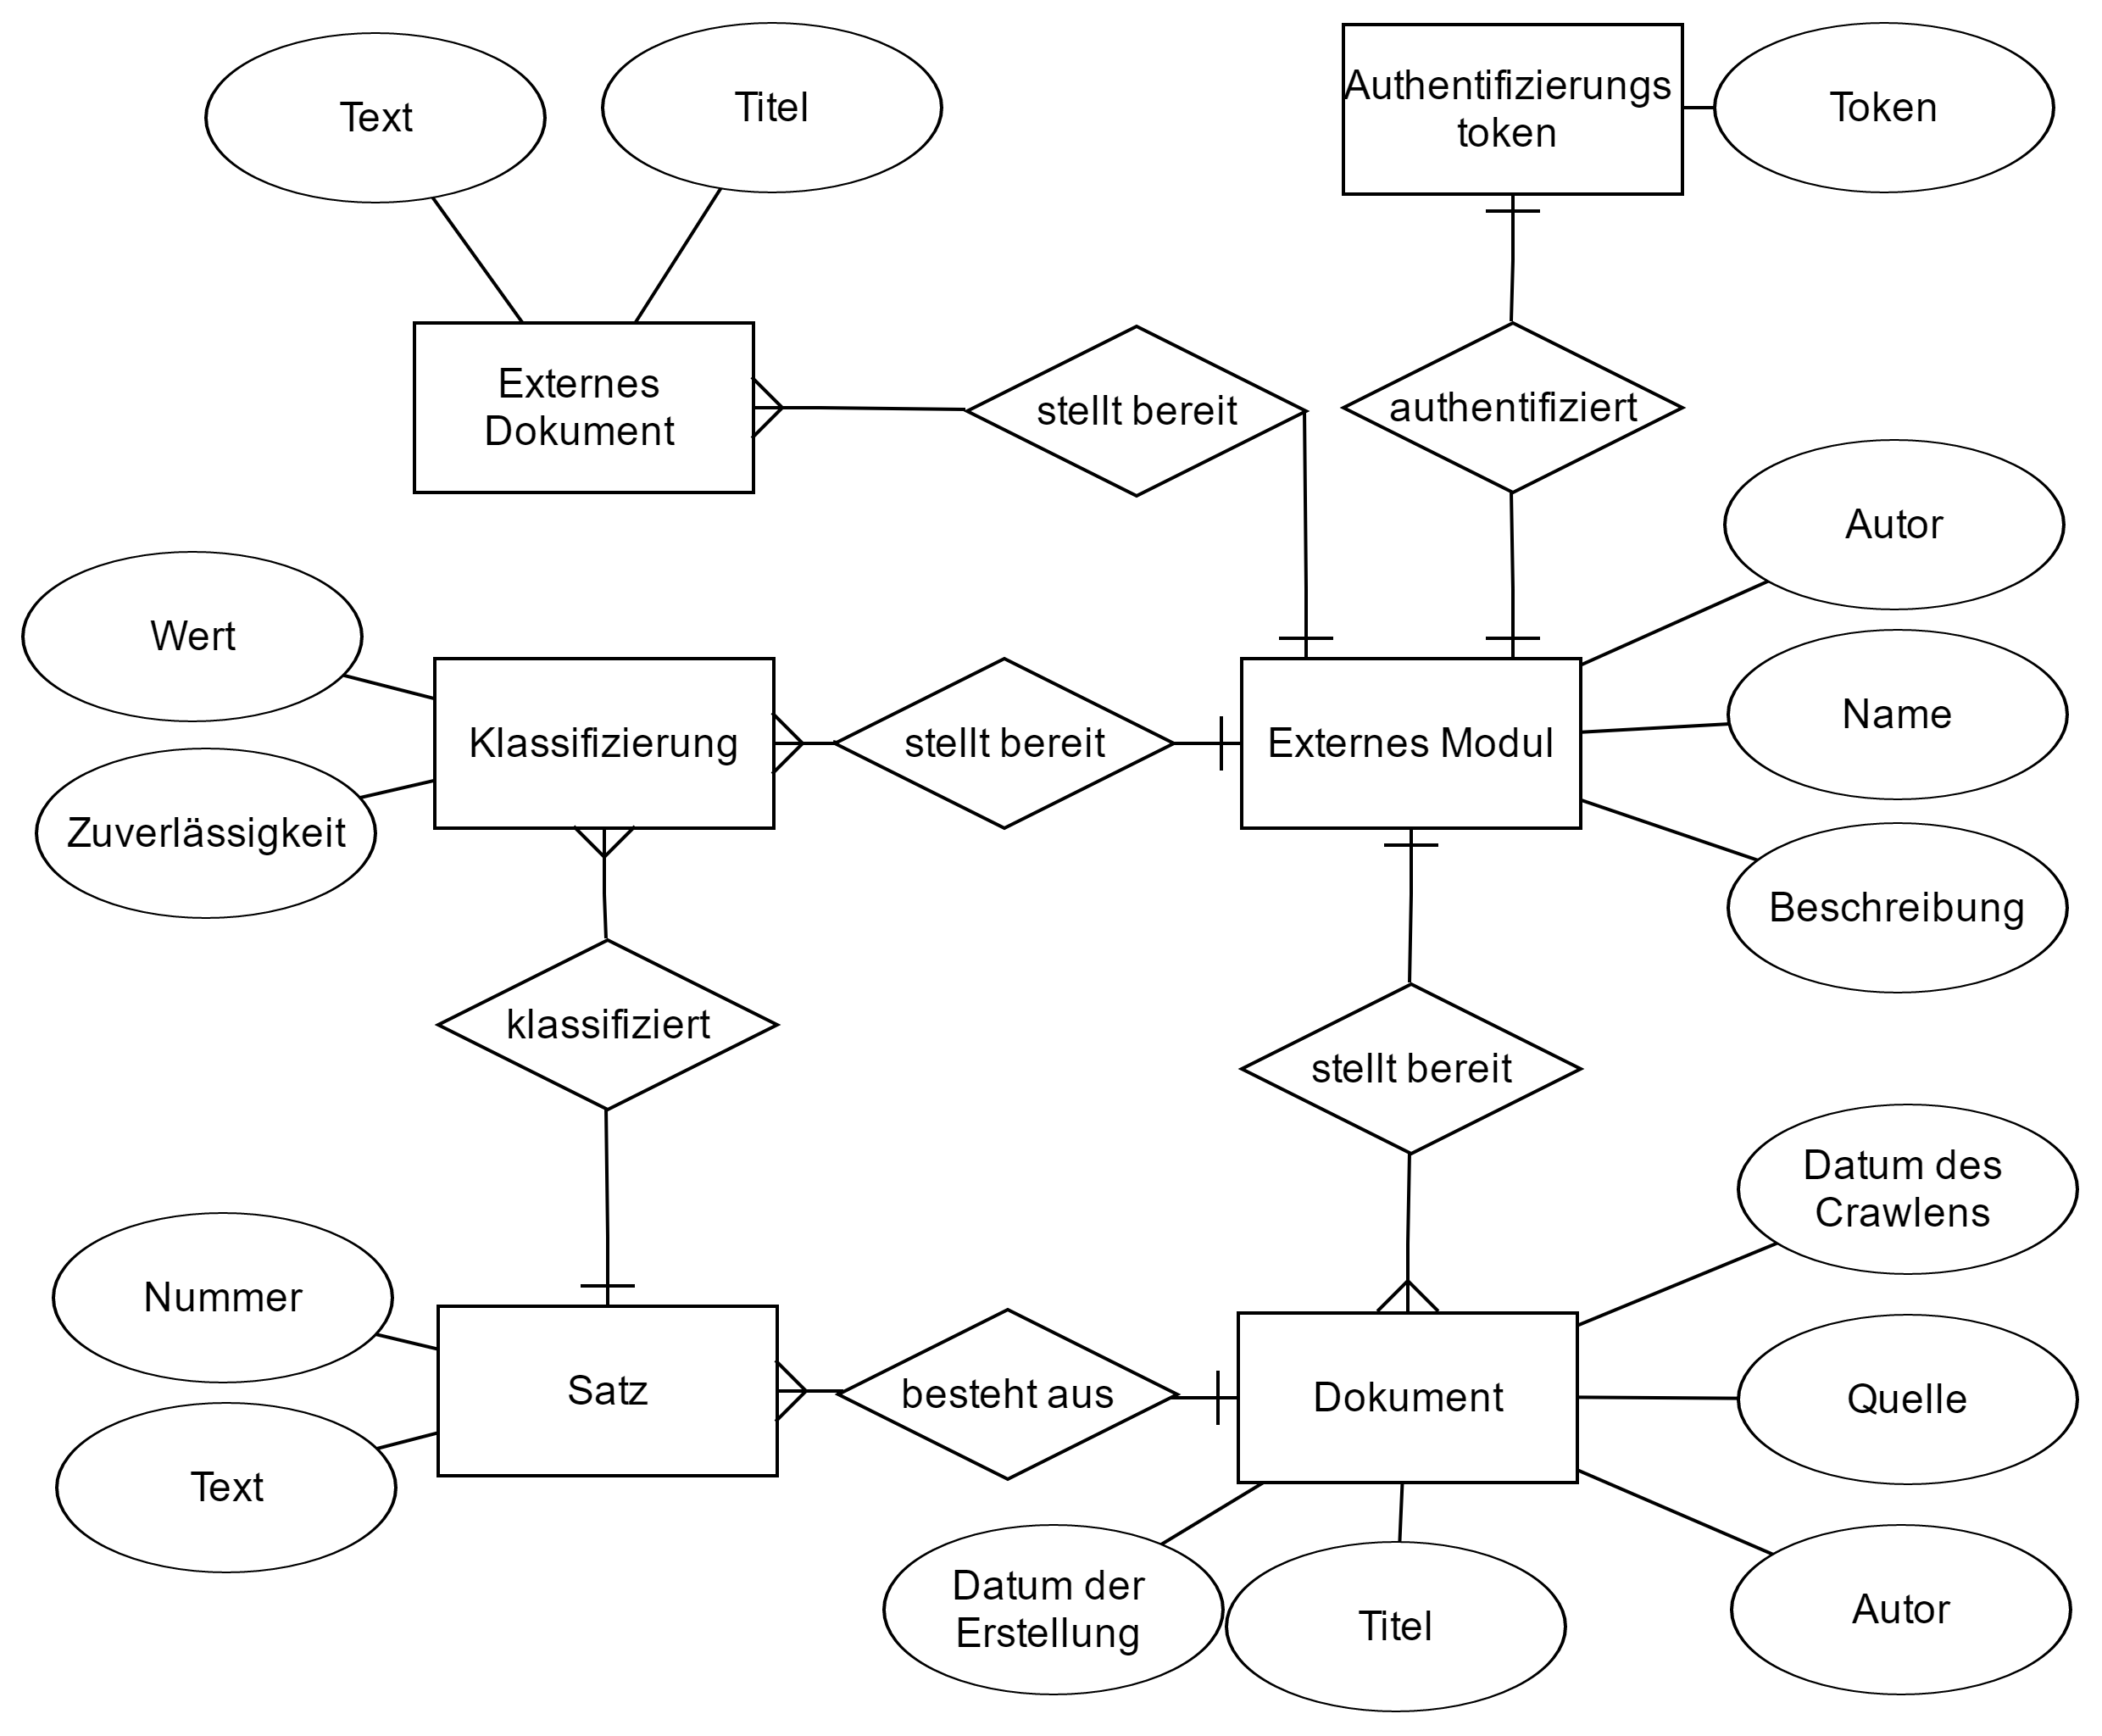
\includegraphics[scale=0.175]{content/erd.png}
	\caption{ERD des Newsboards}
	\label{erd}
\end{figure}

\newpage
Wie aus dem ERD ersichtlich, besteht das Newsboard aus diesen nun näher beschriebenen 
Entitäten:
\begin{itemize}
	\item \textbf{Externe Module}\\
	Die externen Systeme, die Daten für das Newsboard hochladen, werden in dieser Entität
	abgebildet. Von Interesse sind Informationen über den Autor des Moduls,
	den Namen sowie eine kurze Beschreibung.
	\item \textbf{Authentifizierungstoken}\\
	Authentifizierungstokens dienen zur Bestätigung der Identität von externen Modulen.
	Nur Module, die über ein gültiges Authentifizierungstoken verfügen, dürfen in der Lage
	sein, Daten für das Newsboard hochzuladen. Ein Token besteht aus einer zufälligen
	Zeichenkette.
	\item \textbf{Dokumente}\\
	Nachrichten und Texte, die im Newsboard dargestellt werden sollen oder zur
	Klassifizierung bereitstehen, werden als Dokumente im System abgelegt. Der Text wird in
	Sätze aufgeteilt, über die Dokumente werden einige Metainformationen gespeichert. Hierzu
	zählen zum Beispiel das Datum der Erstellung und des Crawlens, der Autor sowie der Titel
	und die Quelle des Dokumentes.
	\item \textbf{Externe Dokumente}\\
	Dokumente oder Nachrichten, die nicht klassifiziert, dem Gesamtsystem aber dennoch zur
	Verfügung stehen sollen, werden als externe Dokumente gespeichert. Der Inhalt dieser
	Dokumente wird als Plaintext abgelegt. Auch der Titel des Dokumentes ist von Interesse.
	\item \textbf{Sätze}\\
	Die eigentlichen Sätze, die in einem Dokument geschrieben sind, werden separat 
	gespeichert. Sie sind es auch, die zur Klassifizierung von externen Modulen 
	bereitstehen. Um ein Dokument wieder korrekt zusammenzusetzen, wird zu dem die 
	Position eines jeden Satzes im Dokument als Nummer gespeichert.
	\item \textbf{Klassifizierungen}\\
	Die Klassifizierungen der Sätze werden in Form dieser Entität gespeichert. Neben den 
	Informationen, zu welchem Satz eine Klassifizierung gehört, muss zudem das 
	klassifizierende Modul abgelegt werden. Sie besteht aus zwei
	Werten: einem für die errechnete Klassifizierung und einem für die Zuversichtlichkeit
	des Moduls. 
\end{itemize}

\subsection{Schnittstelle}
Die Hauptziele bei der Konzeption der Schnittstelle sind zum einen eine möglichst
einfache Verwendung, zum anderen eine verlässliche Validierung der übertragenen Daten.
Da die Schnittstelle auf HTTP aufbaut, bietet es sich an, mit einer REST-Schnittstelle
die Möglichkeiten von HTTP zu nutzen und auf eine zusätzliche Zwischenschicht
zu verzichten.

Als Datenformat für REST-Schnittstellen sind sowohl JSON, als auch XML etabliert.
Da XML im Gegensatz zu JSON allerdings eine verlässliche Möglichkeit zur Validierung
und Dokumentation durch ein Schema besitzt, ist es in diesem Fall die bessere Wahl.
Der geringfügig höhere Speicherverbrauch, sowie die derzeit geringe Popularität
von XML sollen hier keine Rolle spielen.

Bei der Konzeption der verwendeten REST-Ressourcen, sowie deren akzeptierten Methoden,
bestehen ebenfalls zwei mögliche Szenarien. Das erste ist die Abbildung sämtlicher
Datentypen des Datenmodells und das Erlauben aller CRUD-Operationen.
Das zweite Szenario ist es, ausschließlich einige wenige Ressourcen zur Verfügung
zu stellen, welche die geplanten Anwendungsfälle abbilden.

Letzteres verlangt komplexere Daten, die von der Schnittstelle verarbeitet werden müssen,
andernfalls läge diese Komplexität jeweils in den einzelnen Clients und müsste
mehrfach konzeptioniert und umgesetzt werden. Das führt letztendlich zu mehr
unnützer Arbeit und gleichzeitig zur mehr möglichen Fehlerquellen.
Da für diese Schnittstelle potentiell regelmäßig neue Clients entwickelt werden sollen,
ist die zweite Variante als deutlich zweckmäßiger sowie allgemein eleganter anzusehen.

Die sich aus den Anwendungsfällen und konzeptionellen Vorüberlegungen resultierenden
Aktionen, welche durch die REST-Schnittstelle ermöglicht werden, lauten wie folgt:
\begin{itemize}
	\item Einfügen neuer Dokumente
	\item Lesen von Dokumenten
	\item Einfügen neuer Klassifizierungen für Dokumente
\end{itemize}


\section{Implementierung}
Nach dem Konzept wird nun dessen konkrete Umsetzung behandelt,
um einen tieferen Einblick in die Funktionsweise des Newsboards zu geben.

\subsection{Technische Basis}
Umgesetzt wird das Newsboard in Java, sowohl wegen persönlicher Präferenzen der Autoren,
als auch auf Grund der Tatsache, dass hauptsächlich Java als Programmiersprache
an der FH Bielefeld gelehrt wird. So werden der Weiterentwicklung des Newsboards
durch weitere Studenten keine vermeidbaren Hürden in den Weg gestellt.
Darüber hinaus gibt es für Java eine große Zahl an ausgereiften
und gut dokumentierten Bibliotheken sowie verlässliche Frameworks zum 
Build-Management. Verwendet wird das aktuelle Feature-Level von Java 8,
da es keinerlei Altlasten gibt, auf die Rücksicht genommen werden müsste.

Als Basis für das Newsboard wird das Spring-Framework im Zusammenspiel mit Maven
als Build-Management-Tool verwendet. Diese Kombination ist in der Praxis bewährt,
ist flexibel für verschiedenste Anwendungsfälle, sowie ohne große Einarbeitungszeit
gut zu benutzen. Außerdem besteht so keinerlei Bindung
an eine bestimmte Entwicklungsumgebung.

Spring bietet außerdem eine sehr ausgereifte Inversion-of-Control bzw.
Dependency Injection, wodurch eine lose Kopplung der einzelnen Komponenten
untereinander gewährt wird\cite{fowler-ioc}.
In der Umsetzung von Spring werden dabei die einzelnen Klassen nur mit
Annotationen versehen und haben ansonsten keine zwingenden Abhängigkeiten
zum Spring Framework.

Darüber hinaus können neben konkreten Klassen auch Abhängigkeiten zu Interfaces
injiziert werden, welche wiederum in ihrer Auflösung in konkrete Klassen
durch die Konfiguration von Spring beeinflusst werden können.
So kann zum Beispiel entweder eine Konfiguration für eine SQL-Datenbank,
oder einen anderen Datenspeicher angelegt werden und in Abhängigkeit
der aktivierten Konfiguration wird eine andere Implementierung für das
Interface injiziert.

\subsection{Datenmodell}
Das Datenmodell des Newsboards wird mit dem relationalen Datenbankmanagementsystem MySQL
abgebildet. Als weitverbreitetes Open-Source Produkt eignet es sich optimal, um im
Newsboard eingesetzt zu werden. Basierend auf dem vom ERD beschriebenen Modell
(Abb. \ref{fig:erd}) des Newsboards wurde ein physisches Modell für MySQL entwickelt
(Abb. \ref{fig:physical_model}).

\begin{figure}[h]
	\centering
	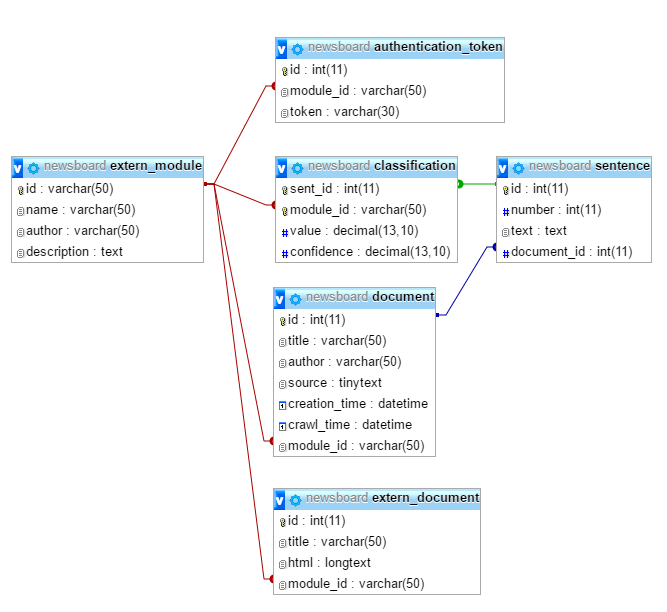
\includegraphics[scale=0.8]{content/physical-model.png}
	\caption{Physisches Modell des Newsboards}
	\label{fig:physical_model}
\end{figure}

Das Modell wird in der Schnittstelle über acht Klassen abgebildet (Abb. 
\ref{fig:uml_model}). Hier zeigen sich Abweichungen zum physischen Modell. So ist die Klasse
Document eine Containerklasse, die die Metainformationen und die Sätze des Dokuments
speichert. Um die Metainformationen eines Dokumentes zu struktieren, ist für sie eine eigene
Klasse vorhanden: DocumentMetaData. Für Sätze steht die Klasse Sentences bereit, die zudem
eine Liste mit allen Klassifikationen eines Satzes beinhaltet. Die  Klasse RawDocument dient
rein zum Einlesen von Dokumenten, welche von Crawlern bereitgestellt werden. Sie besteht aus
den Metainformationen und dem Text eines Dokumentes. Nach dem Einlesen wird ein RawDocument
in ein Document überführt.

\begin{figure}[h]
	\centering
	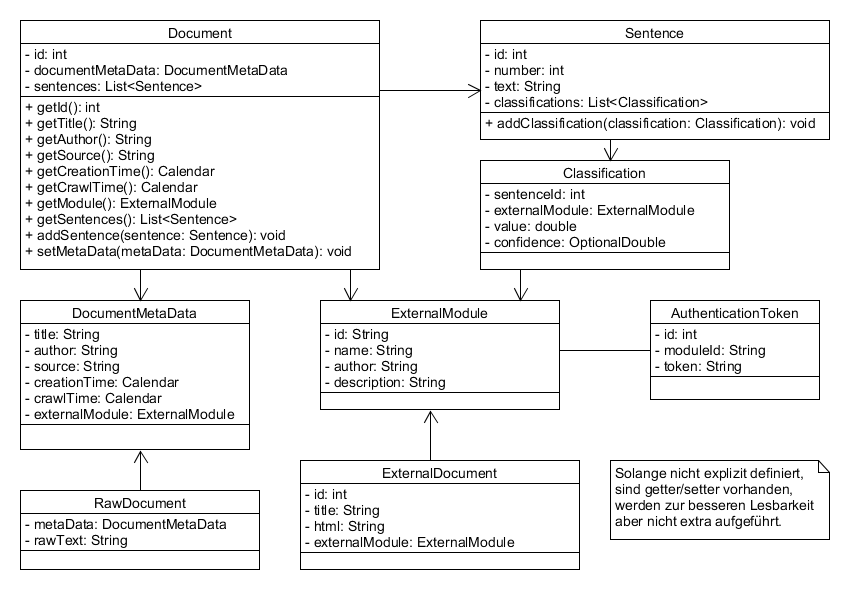
\includegraphics[scale=0.5]{content/uml-model.png}
	\caption{Diagramm der intern verwendeten Modellklassen}
	\label{fig:uml_model}
\end{figure}

Für die Kommunikation zwischen der Schnittstelle und der Datenbank wird auf das
Data-Access-Object Design Muster gesetzt, um eine hohe Modularität und Flexibilität zu
gewährleisten \cite{dao-pattern}. Beim DAO Muster werden verschiedene Interfaces
verwendet, um den Zugriff auf Datenbankoperationen zu maskieren, während die eigentliche
Übertragungslogik pro Datenquelle eigens entwickelt werden kann. Das, und die
Dependency-Injection von Spring, ermöglichen es, im Falle eines Datenbankwechsels von
MySQL hin zu einem beliebigen anderem System, die Schnittstelle fast ohne Anpassungen
weiter verwenden zu können.

\subsection{Dokumentverarbeitung}
Um die RawDocuments, welche von Crawlern über die REST-Schnittstelle eingefügt werden,
in Document-Objekte zu überführen, muss der Text in einzelne Sätze aufgeteilt werden.
Diesen Zweck erfüllt die Klasse RawDocumentProcessor. Sie nutzt die
Apache openNLP Bibliothek, um den unverarbeiteten Text von RawDocuments in Sentences zu
überführen.

Apache openNLP ist eine Sammlung verschiedener Werkzeuge, um mit Java einfach diverse 
NLP-Probleme zu lösen \cite{opennlp}. Es liefert neben unterschiedlichen 
Machine-Learning-Algorithmen auch fertige Modelle zur Verwendung mit, unter anderem
zum Finden von einzelnen Sätzen. Diese Modelle sind in verschiedenen Sprachen vorhanden,
für das Newsboard wird eines zur Erkennung der deutschen Sprache genutzt.

OpenNLP stellt zur Satzerkennung das Interface SentenceDetector und die davon ableitende
Klasse SentenceDetectorME zur Verfügung. SentenceDetectorME nutzt ein Maximum-Entropy-Modell
zur Klassifizierung von Satzzeichen, die einen Satz beenden. Sie wird auch im
RawDocumentProcessor eingesetzt. Über einen einfachen Methodenaufruf kann so ein kompletter
Text verarbeitet werden. Auch die Kopplung zu openNLP bleibt sehr gering, da die
Bibliothek nur hier Verwendung findet.

\subsection{Schnittstelle}
Zur Implementierung der REST-Endpoints der Schnittstelle werden die in Spring enthaltenen
Controller-Features genutzt. Um damit einen Endpoint zu bedienen, reicht es aus,
eine Methode innerhalb einer Controller-Klasse mit \texttt{RequestMapping} zu annotieren.
Listing \ref{lst:restExample} zeigt beispielhaft, wie ein solcher Endpoint unter Angabe der
Annotations-Parameter implementiert werden kann.

Der Rückgabewert der Methode wird so direkt als Antwort an den Client zurückgeliefert.
Darüber hinaus können mit Hilfe der Dependency-Injection von Spring weitere Parameter
definiert werden, wie die HTTP-Anfrage oder eine Antwort wie der im Beispiel.
\vspace{1em}

\begin{java}{Implementierung eines REST-Endpoints mit Spring}{lst:restExample}
@RestController
public class RestApiController {
	[...]
	@RequestMapping(path = "/document", method = RequestMethod.GET, produces = MediaType.APPLICATION_XML_VALUE)
	public String listDocuments(HttpServletResponse response) {
		[...]
		return documents;
	}
	[...]
}
\end{java}

Auf diese Weise werden jeweils die im Konzept aufgezählten Aktionen implementiert.
Es ergeben sich zur wesentlichen Vereinfachung der Benutzung der Schnittstelle,
sowie um möglichst effektiv arbeiten zu können, mehrere Endpoints zum Lesen
der Dokumente. Somit bildet sich die folgende Liste an vorhandenen
Kombinationen von Aktionen und Ressourcen:

\begin{itemize}
	\item \textbf{GET /document}
	Lesen einer Liste der Metadaten aller Dokumente
	\item \textbf{GET /document/\{id\}}
	Lesen eines vollständigen, spezifizierten Dokuments inklusive
	einzelnen Sätzen und Klassifikationen
	\item \textbf{PUT /document}
	Einfügen eines neuen Dokuments durch einen Crawler
	\item \textbf{GET /unclassified}
	Lesen aller Dokumente, die vom aktuell authentifizierten Classifier
	noch nicht bewertet wurden
	\item \textbf{PUT /classify}
	Einfügen neuer Klassifizierungen durch einen Classifier
\end{itemize}

Um die Ressourcen der REST-Schnittstelle klar von der Web-Oberfläche zu trennen,
sind die angegebenen Pfade relativ zum Verzeichnis \texttt{/rest}.

Da nicht jeder beliebige Nutzer neue Dokumente oder Klassifizierungen einfügen
können soll, muss eine Art von Authentifizierung vorhanden sein.
Es bietet sich an, auch das Lesen von unklassifizierten Dokumenten nur authentifizierten
Nutzern zugänglich zu machen, da dies immer spezifisch
für einen bestimmten Classifier ist.
Umgesetzt wird dies mit einer HTTP-Basic Authentifizierung, die sehr einfach umzusetzen
ist, aber für die vorgesehenen Einsatzzwecke ausreicht.
Als Benutzername dient immer die ID des Crawlers oder Classifiers, die in der Datenbank
hinterlegt ist. Als Passwort dient ein in der Datenbank hinterlegtes AuthenticationToken.

\subsection{XML-Format}
Über die REST-Endpoints hinaus ist bei der Schnittstelle noch die Verarbeitung
der XML-Daten, sowie das Schema zur Validierung interessant.
Da die zu erwartenden Datenmengen im Vorhinein nicht abschätzbar sind,
sollte das Lesen und vor allem das Schreiben der XML-Daten möglichst wenig Speicher
verbrauchen, um eventuelle Engpässe zu vermeiden. Beim Lesen ist eine Validierung
gegen das Schema unbedingt notwendig, da nicht davon ausgegangen werden kann,
dass die ankommenden Daten in jedem Fall valide sind.

Aufgrund der Speicheranforderungen ist ein herkömmlicher DOM-Parser in diesem Projekt
nicht geeignet. Gelesen werden die XML-Daten stattdessen mit einem SAX-Parser\cite{insel-xml}. Dieser ist weniger speicherbelastend als ein DOM-Parser
und kann, anders als ein StAX-Parser, eine Validierung des Dokuments während
des Einlesens durchführen. Verwendet wird die Standard Implementierung
des JDK: \texttt{javax.xml.parsers.SAXParser}.

Da SAX-Parser üblicherweise nur lesen, aber nicht schreiben können, kommt dazu ein
anderer Parser zum Einsatz. In diesem Fall ein StAX-Parser,
da Validierung nicht zwingend zur Laufzeit erfolgen muss, sondern im Vorhinein
im Zuge automatisierter Tests durchgeführt werden kann.
Verwendet wird hier ebenfalls eine Implementierung, die Bestandteil des JDK ist:
\texttt{javax.xml.stream.XMLStreamWriter}.
Um die genauere Arbeitsweise beim Verarbeiten der XML-Daten zu beschreiben,
wird an dieser Stelle das erstellte Schema beschrieben.

Das im Schema spezifizierte XML-Format erlaubt Dokumente verschiedenster Ausprägung.
Das ist notwendig, damit einerseits nicht mehrere Schemata angelegt und gepflegt
werden zu müssen, und andererseits die Anforderungen der verschiedenen
REST-Endpoints erfüllt werden.

Das Schema ist so spezifiziert, dass jedes XML-Dokument eine Liste von Dokumenten
im Sinne des Datenmodells enthalten kann.
Dabei kann jedes Dokument Metadaten enthalten (z.B. Autor, Quelle), die beim Einlesen
neuer Dokumente und beim Ausgeben vorhandener Dokumente angegeben sein müssen.
Dazu kommt entweder ein Element mit Rohtext beim Einfügen der Dokumente,
oder eine Liste von Sätzen und Klassifikationen.

Die Sätze sind nur beim Ausgeben von Dokumenten wichtig, beim Einlesen
neuer Klassifikationen sind sie, wie die Metadaten auch,
optional und werden nicht beachtet.
Wenn eine Liste von Sätzen vorhanden ist, muss sie mindestens einen Satz enthalten.
Die Liste von Klassifikationen ist beim Ausgeben spezifizierter
und unklassifizierter Dokumente von Belang, sowie natürlich
beim Einlesen neuer Klassifikationen. Da z.B. bei frisch eingelesenen Dokumenten noch keine Klassifizierungen vorliegen können, darf die Liste auch leer sein.

Um das Arbeiten mit diesen Dokumenten deutlich zu vereinfachen, können XML-Dokumente
weder in beliebiger Ausprägung geschrieben noch gelesen werden. Stattdessen können
nur XML-Daten eingelesen werden, wie sie zum Einfügen neuer Dokumente
oder Klassifizierungen notwendig sind.
Geschrieben werden können nur Dokumentenausschnitte (intern Stub genannt),
die nur Metadaten beinhalten, oder vollständige Dokument-Strukturen.

\subsection{Web-Oberfläche}
Um das Newsboard über die REST-Schnittstelle hinaus auch für Benutzer verfügbar zu machen,
beinhaltet es eine einfache Web-Oberfläche.
Diese ist im jetzigen Zustand nur im Stande, eine Liste von klassifizierten Dokumenten,
oder eine Detailseite zu einem einzelnen Dokument anzuzeigen.

Auf der Übersichtsseite werden nur Titel, Inhalt und ein berechneter Durchschnittswert
aller Klassifikationen zu einem Dokument angezeigt. Auf der Detailseite werden
darüber hinaus noch weitere Metadaten, wie Quelle, Crawler, Einlesezeitpunkt
und, wenn verfügbar, auch Autor und Veröffentlichungsdatum angezeigt.

Die Durchschnittsberechnung ergibt sich, indem zu jedem Satz einzeln ein Durchschnitt
berechnet wird und anschließend das arithmetische Mittel aller Satzbewertungen
gebildet wird. Die Satzbewertungen werden berechnet, indem ebenfalls das arithmetische
Mittel aller vorliegenden Bewertungen gebildet wird. Falls vorhanden, wird dabei auch der
Wert für die Zuversichtlichkeit mit einbezogen, indem er mit dem jeweiligen
Klassifikationswert multipliziert wird.

Bei der Oberfläche handelt es sich um eine klassische, serverseitig generierte.
Dabei wird die Thymeleaf-Template-Engine verwendet, für die es eine einfach Integration in
Spring gibt. Sie verfolgt den sogenannten "`Natural Templating"'-Ansatz,
bei dem die HTML-Templates auch in ihrer Rohfassung korrekt von einem Browser
dargestellt werden können. Dadurch ist allerdings das Ausgabeformat
auf HTML-Dialekte beschränkt.

Um die Oberfläche mit geringem zusätzlichen Aufwand optisch ansprechend zu gestalten,
kommt das Bootstrap-Framework zum Einsatz. Es wird von Twitter entwickelt und
beinhaltet viele Möglichkeiten, Layouts zu gestalten und einfache Inhalte
ansehnlich darzustellen\cite{bootstrap}.

\subsection{Testing}
Um eine korrekte Funktion des Newsboards zu gewährleisten und möglichst früh
Fehler zu erkennen, wurde zu großen Teilen testgetrieben entwickelt.
Als Testing-Framework kam Spock zum Einsatz. Es bietet gegenüber JUnit einige Vorteile,
wie das Strukturieren von Testfällen in given/when/then-Blöcke,
oder das, durch die Programmierung in Groovy ermöglichte, Testen privater Methoden
außerhalb der entsprechenden Klassen.

Zusätzlich kam das JaCoCo-Maven-Plugin zum Einsatz, um die Testabdeckung des Newsboards
zu messen. In der finalen Fassung liegt die Zeilenabdeckung bei 92\%
und die Entscheidungsabdeckung bei 76\% für das gesamte Projekt.
Für die Model-Klassen besteht darüber hinaus vollständige Zeilenabdeckung,
sowie 89\% Entscheidungsabdeckung. Dabei ist zu beachten, dass JaCoCo einige Pfade
mit einberechnet, die sich gegenseitig ausschließen, und entsprechend
nicht abgedeckt werden können. Ein Beispiel dafür ist die oder-verknüpfte Abfrage
auf Null und eine Klassenzugehörigkeit, die mehrfach in \texttt{equals}-Methoden vorkommt.


\section{Schluss}
\subsection{Zusammenfassung}

\subsection{Ausblick}
Zurückblickend hat sich die Entwicklung des Newsboards als erfoglreich gezeigt. Durch die
Verwendung von Spring, Java und MySQL als Grundlage konnte eine modulare, flexible und 
performante Software entwickelt werden. Darüber hinaus bietet das Newsboard weitere
Ansatzpunkte zur Entwicklung neuer Funktionalitäten. Neben der Erweiterung der REST-
Schnittstelle mit zusätzlichen Optionen ist auch eine überarbeitete und umfangreichere 
Oberfläche denkbar, die in späteren Studentenprojekten entwickelt werden können.
\\ \\
Auch eine Verwendung von weiteren Datenbanksystemen ist denkbar. Mit den fortschreitenden
Entwicklungen im Bereich der NoSQL-Datenbanken ist es durchaus möglich, dass, in absehbarer
Zeit, eine Alternative zum relationalen Modell eingesetzt werden kann. 


%% zusammenfassung & Ausblick

%% Ausblick: weitere themen könnten die implementierung dieses konzept in ein Chef-Script / XYZ Script sein

%Appendix

\cleardoublepage
\phantomsection
\addcontentsline{toc}{section}{\bibname}
\bibliography{literatur}

\end{document}